\documentclass{article}


\usepackage{verbatim}
\usepackage[utf8]{inputenc}
\usepackage[portuges,portuguese]{babel} 


% para que o índice possa ter o título de ``Índice'' (caso contrário fica ``Conteúdo'')
\addto\captionsportuguese{% Replace "english" with the language you use
  \renewcommand{\contentsname}%
    {Índice}%
}
\usepackage[nottoc,notlot,notlof]{tocbibind}

% para a inclusão de figuras
\usepackage{graphicx}

% para que não haja indentação no início dos parágrafos
\setlength{\parindent}{0pt} 

% para que os links apareçam como hiperligações
\usepackage{url}
\usepackage{hyperref}

\usepackage[usenames,dvipsnames]{color}    
%para introduzirmos fragmentos de script de R (ou de outra linguagem de programação)
\usepackage{listings} %para inserir excertos de codigo

\usepackage{subfigure} %Para incluir figuras lado a lado

\newcommand*{\authorimg}[1]{\raisebox{-.0\baselineskip}{\includegraphics[height=12pt,width=12pt,keepaspectratio,]{#1}}} %Para inserir o símbolo do R

\lstset{ 
  language=R,                     % linguagem
  basicstyle=\small\ttfamily, % tamanho das fontes usadas
  numbers=left,                   % onde colocar numeração das linhas de código
 numberstyle=\tiny\color{blue},  % estilo a usar para numeração das linhas
  stepnumber=1,                   % distância entre duas linhas numeradas (se for 1, cada linha será numerada)
  numbersep=5pt,                  % distância a que a numeração das linhas está do código
  backgroundcolor=\color{white},  % cor do background
  showspaces=false,               
  showstringspaces=false,         % sublinhar espaços em strings
  showtabs=false,                
  frame=single,                   % coloca uma moldura à volta do código
  rulecolor=\color{black},        % cor do frame
  tabsize=2,                    
  captionpos=b,                   % posição da legenda
  breaklines=true,                % line breaking automático
  breakatwhitespace=false,        
  keywordstyle=\color{RoyalBlue},      % estilo das keywords
  commentstyle=\color{YellcowGreen},   % estilo dos comentários
  stringstyle=\color{ForestGreen}      % estilo das strings
} 
%%%%%%% INÍCIO DO DOCUMENTO %%%%%%%
\begin{document}
\thispagestyle{empty}
% CAPA
\begin{flushleft}

\includegraphics[scale=0.15]{ESTB.jpg}
\end{flushleft}

\begin{center}
\Large{Instituto Politécnico de Setúbal}
\end{center}

\begin{center}
\Large{Escola Superior de Tecnologia do Barreiro}
\end{center}

\medskip % para dar um espaço vertical


\begin{center}
\Large{\textbf{Trabalho de Grupo Projeto de Introdução à Estatística}}
\end{center}
\begin{center}
\Large{Licenciatura em Bioinformática}
\end{center}

\vspace{3cm} % espaço vertical (uma alternativa ao \medskip, que pode ser customizada para efeitos estéticos)

\begin{center}
\huge{\textbf{Estudo estatístico sobre }} 
\end{center}


\begin{center}
\Large{Junho de 2022}
\end{center}

\medskip
\begin{center}
\large{Grupo 07}

\large{João Almeida (202100068)}

\large{Pedro Pacheco (202100957)}

\large{Hélder Marques (202100959)}

\large{Guilherme Parreira (202100206)}

\end{center}

% FIM DA CAPA

\newpage
\pagenumbering{roman}
%\phantomsection

% Página com o índice
\tableofcontents

\newpage
\pagenumbering{arabic}

%%%%%%% SECÇÃO "INTRODUÇÃO" %%%%%%%
\section{Introdução}\label{sec:introducao} % a label pode ser o que se quiser

Neste projeto vamos realizar uma análise descritiva univariada e bivariada sobre 3 (três) espécies de flor: \textit{Ranunculus sp.}, \textit{Geranium sp.}, \textit{Crepis sp.}, o seu número, comprimento e largura das pétalas, cor (amarelo e roxo) e humidade.  
Vamos abordar o comprimento e a largura das pétalas por espécie e a humidade por cor da pétala e por espécie. Vamos também analisar o tipo de espécie em relação ao comprimento da pétala e a correlação entre largura da pétala e humidade. Em todas estas análises incluiremos tabelas e gráficos, assim como também todos os cálculos realizados para fundamentar as mesmas.

%%%%%%% SECÇÃO "DESENVOLVIMENTOS" %%%%%%%

\section{Metodologia}\label{sec:metodologia}

\subsection{Conceitos utilizados}
Desenvolvemos este projeto com recurso à análise estatística.
Análise estatística permite recolher, explorar, organizar e apresentar grandes quantidades de dados. Desenvolvemos estas atividades através de testes de hipóteses, análise exploratória e modelação de dados. Utilizámos uma população alvo que é um conjunto de individuos sobre os quais é efetuada uma avaliação e/ou uma análise estatística.
\subsection{População alvo e variáveis}
\paragraph{} A nosssa população de estudo é constituida por 150 (cento e cinquenta) amostras das seguintes espécies C{Ranunculus sp.}, \textit{Geranium sp.}, \textit{Crepis sp.} Para avaliar a nossa população alvo utilizámos as seguintes variáveis: Tipo de espécie (\textit{Ranunculus sp.}, \textit{Geranium sp.}, \textit{Crepis sp.}) ; Cor (Amarelo e Roxo); Nº pétalas; Comprimento das Pétalas; Largura das Pétalas.

\subsection{Análise estatística}

\paragraph{} Para esta população utilizámos análise univariada e bivariada. A análise univariada analisa a distribuição e dispersão dos dados, inclui a análise dos valores da média, moda, mediana e quartis. A  análise bivariada permite observar como duas variáveis se comportam na persença uma da outra, ou seja a sua associação, correlação e dependência.

\paragraph{} No nosso projeto utilizámos todas as medições estudadas da estatistica univariada, ou seja, média, mediana, moda e quartis. Em relação à análise bivariada utilizámos a associação de Cramer e a correlação de Pearson.

Utilizámos a associação de Cramer porque são utilizadas duas variáveis qualitativas numa tabela de contigência. A correlação de Pearson foi utilizada para nos ser permitido realizar a análise entre duas variáveis quantitativas.

\section{Caracterização da amostra}\label{sec:caracterizacao_amostra}

\subsection{Análise Descritiva Univariada e Bivariada}

\subsubsection{Análise do comprimento das pétalas por espécie(Bivariada)}

\begin{figure}[h]
       \centering %centrar
        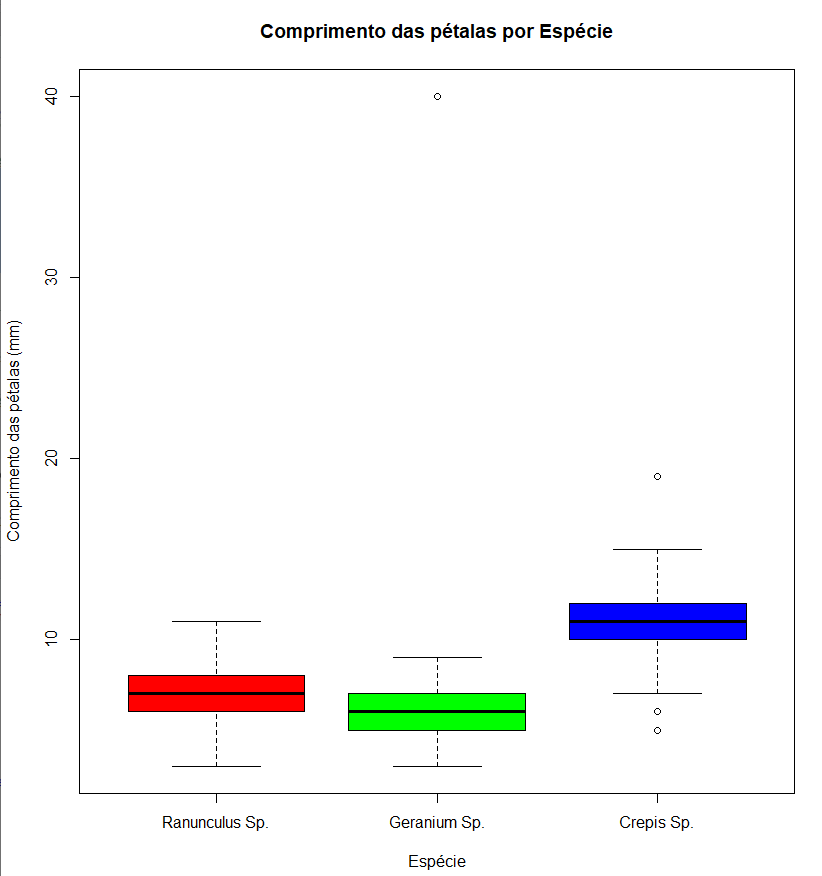
\includegraphics[scale=0.6]{analise comprimento por especie.png}
       \caption{Análise do comprimento das pétalas por espécie.}
       \label{fig:logo}
    \end{figure}
    
\paragraph{} Como podemos observar neste grafico o comprimento das pétalas (por mm) tem uma pequena divergência de espécie para espécie. Sendo que a espécie \textit{Crepis Sp} apresenta em média o maior comprimento de pétalas entre as tres (3) espécies, e também podemos observar que a espécie \textit{Geranium sp} tem em média o menor comprimento de pétala entre as tres (3) espécies.

\paragraph{}\textit{Ranunculus sp}: Valor minimo de 3.0 e máximo de 11.0, primeiro quartil de 6.0, mediana de 7.0, média de 7.1,  terceiro quartil 8.0, variência de 2.33, desvio-padrão de 1.53 e com um coeficiente de disperção de 0.213.
\paragraph{} \textit{Geranium sp}: Valor minimo de 3.0 e máximo de 5.0, primeiro quartil de 7.0, mediana de 6.0, média de 6.6,  terceiro quartil 7.0, variência de 25.59, desvio-padrão de 5.06 e com um coeficiente de disperção de 0.765.

\paragraph{} \textit{Crepis Sp}: Valor minimo de 3.0 e máximo de 19.0, primeiro quartil de 10.0, mediana de 11.0, média de 10.620,  terceiro quartil 12.0, variência de 6.77, desvio-padrão de 2.60 e com um coeficiente de disperção de 0.245.

\begin{figure}[h]
       \centering 
        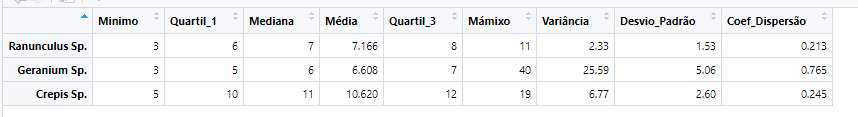
\includegraphics[scale=0.8]{tabela_comprimento_especie.png}
       \caption{Tabela com as medidas de localização e expressão das pétalas por espécie.}
       \label{fig:logo}
    \end{figure}


\paragraph{}
\paragraph{}
\paragraph{}
\paragraph{}
\paragraph{}
\paragraph{}
\paragraph{}
\paragraph{}
\paragraph{}
\paragraph{}
\paragraph{}
\paragraph{}
\paragraph{}
\subsubsection{Análise da largura das pétalas por espécie (Bivariada)}

\begin{figure}[h]
       \centering %centrar
        \includegraphics[scale=0.6]{analise largura por espécie.png}
       \caption{Análise do comprimento do comprimento das pétalas por espécie.}
       \label{fig:logo}
    \end{figure}

\paragraph{} Com a análise deste gráfico podemos compreender que em média a espécie \textit{Ranunculus sp} apresenta uma maior largura de petalas(mm) entre as tres espécies enquanto que \textit{Crepis Sp} apresenta em média a menor largura de pétalas.

\paragraph{}\textit{Ranunculus sp}: Valor minimo de 1.0 e máximo de 7.0, primeiro quartil de 4.0, mediana de 4.0, média de 4.3,  terceiro quartil 5.0, variência de 1.50, desvio-padrão de 1.239 e com um coeficiente de disperção de 0.285.

\paragraph{} \textit{Geranium sp}: Valor minimo de 1.0 e máximo de 20.0, primeiro quartil de 2.0, mediana de 3.0, média de 3.03,  terceiro quartil 3.0, variência de 6.42, desvio-padrão de 2.534 e com um coeficiente de disperção de 0.836.

\paragraph{} \textit{Crepis Sp}: Valor minimo de 0.1 e máximo de 3.0, primeiro quartil de 1.0, mediana de 1.0, média de 1.50,  terceiro quartil 2.0, variência de 0.40, desvio-padrão de 0.638 e com um coeficiente de disperção de 0.422.

\begin{figure}[h]
       \centering %centrar
        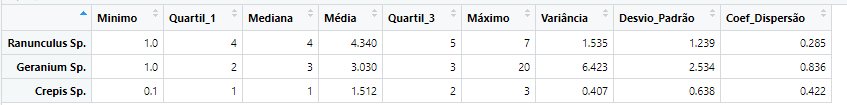
\includegraphics[scale=0.8]{tabela_largura_especie.png}
       \caption{Tabela com as medidas de localização e expressão da largura das pétalas por espécie.}
       \label{fig:logo}
    \end{figure}

\paragraph{}

\paragraph{}
\paragraph{}
\paragraph{}
\paragraph{}
\paragraph{}
\paragraph{}
\paragraph{}
\paragraph{}
\paragraph{}
\paragraph{}
\paragraph{}
\paragraph{}
\paragraph{}
\paragraph{}

\subsubsection{Análise da Humidade das pétalas por cor (Bivariada)}


\begin{figure}[h]
       \centering %centrar
        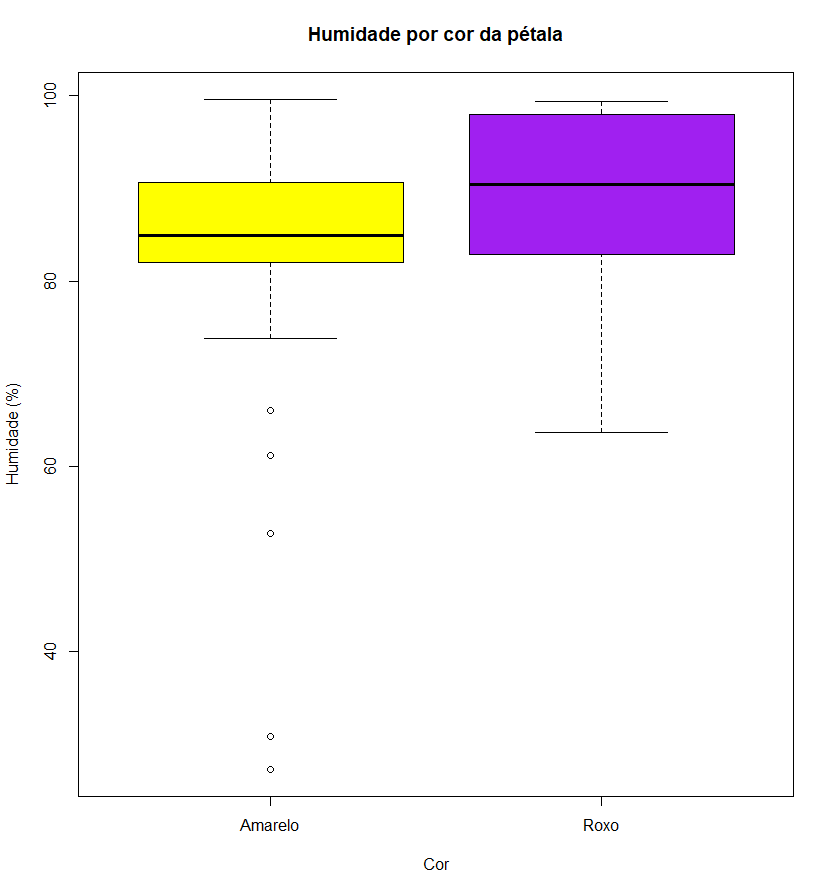
\includegraphics[scale=0.6]{Humidade por cor.png}
       \caption{Análise da Humidade das pétalas por cor.}
       \label{fig:logo}
    \end{figure}

\paragraph{} Com este gráfico podemos inferir que a percentagem de humidade nas pétalas de cor roxa é em média maior que as pétalas de cor amarela e também podemos observar a existência de outliers nas pétalas de cor amarela ou seja existem pétalas de cor amarela com uma baixa percentagem de humidade.

\paragraph{} Amarelo: Valor minimo de 27.27 e máximo de 99.60, primeiro quartil de 81.98, mediana de 84.93, média de 84.76,  terceiro quartil 90.57, variência de 114.898, desvio-padrão de 10.719 e com um coeficiente de disperção de 0.126.

\paragraph{} Roxo: Valor minimo de 63.64 e máximo de 99.41, primeiro quartil de 82.85, mediana de 90.38, média de 88.51,  terceiro quartil 97.98, variência de 87.26, desvio-padrão de 9.341 e com um coeficiente de disperção de 0.105.

\begin{figure}[h]
       \centering %centrar
        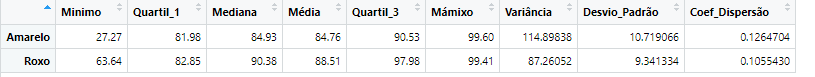
\includegraphics[scale=0.8]{tabela_humidade_cor.png}
       \caption{Tabela com as medidas de localização e expressão das pétalas por cor.}
       \label{fig:logo}
    \end{figure}
    
\paragraph{}

% Humidade por espécie (Bivariada)

\subsubsection{Humidade por espécie (Bivariada)}

\begin{figure}[h]
       \centering %centrar
        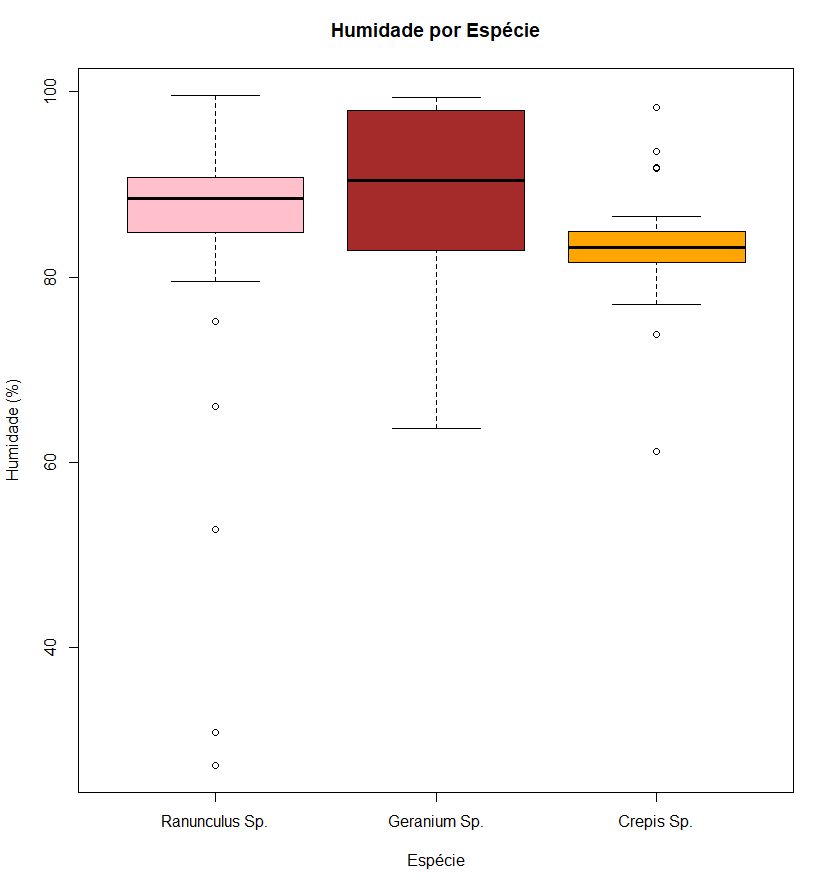
\includegraphics[scale=0.6]{Analise humidade por especie.png}
       \caption{Humidade por espécie}
       \label{fig:logo}
    \end{figure}
    
\paragraph{} Neste grafico podemos inferir que a espécie \textit{Geranium sp} apresenta em média uma maior percentagem de humidade por espécie. Podemos também observar que a espécie \textit{Crepis Sp} apresenta outliers, ou seja, existem petalas desta espécie com maior e com menor percentagem de humidade. Mas a espécie \textit{Ranunculus Sp} também apresenta outliers com percentagem de humidade inferior.

\paragraph{}\textit{Ranunculus sp}: Valor minimo de 27.27 e máximo de 99.60, primeiro quartil de 85.00, mediana de 88.52, média de 85.35,  terceiro quartil 90.70, variência de 195.77, desvio-padrão de 13.992 e com um coeficiente de disperção de 0.164.

\paragraph{} \textit{Geranium sp}: Valor minimo de 63.64 e máximo de 99.41, primeiro quartil de 82.85, mediana de 90.38, média de 88.51,  terceiro quartil 97.98, variência de 87.26, desvio-padrão de 9.341 e com um coeficiente de disperção de 0.106.

\paragraph{} \textit{Crepis Sp}: Valor minimo de 61.15 e máximo de 98.35, primeiro quartil de 81.56, mediana de 83.19, média de 84.16,  terceiro quartil 84.94, variência de 35.64, desvio-padrão de 5.970 e com um coeficiente de disperção de 0.070.

\begin{figure}[h]
       \centering %centrar
        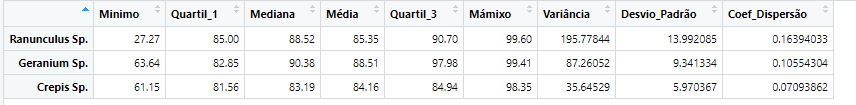
\includegraphics[scale=0.8]{tabela_humidade_especie.png}
       \caption{Tabela com as medidas de localização e expressão da humidade das pétalas por espécie.}
       \label{fig:logo}
    \end{figure}
\paragraph{}
\paragraph{}
\paragraph{}
\paragraph{}
\paragraph{}
\paragraph{}
\paragraph{}
\paragraph{}
\paragraph{}
\paragraph{}

\subsubsection{Gráfico circular para a variável cor (Univariadas)}
\begin{figure}[h]
       \centering %centrar
        \includegraphics[scale=0.6]{Gráfico cor.png}
       \caption{Gráfico circular para a variável cor.}
       \label{fig:logo}
    \end{figure}

\paragraph{} Com a análise deste grafico podemos concluir que a moda é a cor amarela.

\paragraph{} 

\paragraph{}

\paragraph{}

\paragraph{}

\paragraph{}

\paragraph{}

\paragraph{}

\paragraph{}

\subsubsection{Gráfico circular para a variável espécie (Univariadas)}
\begin{figure}[h]
       \centering %centrar
        \includegraphics[scale=0.6]{Grafico espécie.png}
       \caption{Gráfico circular para a variável espécie.}
       \label{fig:logo}
    \end{figure}
    
\paragraph{} De acordo com a analise do gráfico concluimos que a variável espécie não tem moda pois tem a mesma quantidade de cada espécie.

\paragraph{}

\paragraph{}

\paragraph{}

\paragraph{}

\paragraph{}

\paragraph{}

\paragraph{}

\subsubsection{Gráfico para a variável Humidade (Univariadas)}
\begin{figure}[h]
       \centering %centrar
        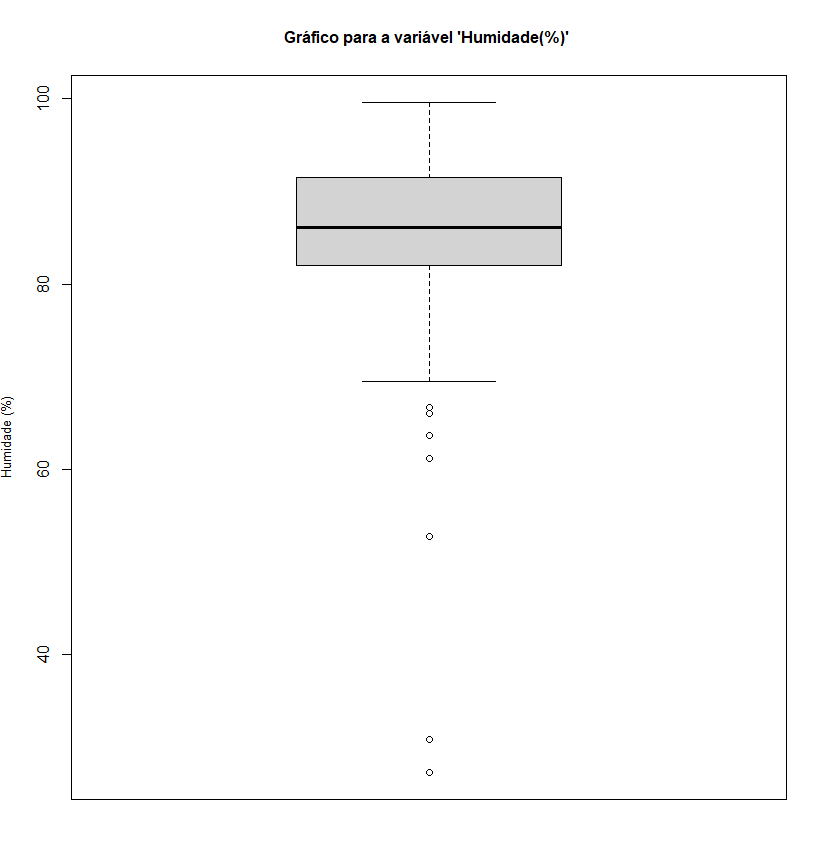
\includegraphics[scale=0.6]{grafico humidade.png}
       \caption{Gráfico para a variável humidade.}
       \label{fig:logo}
    \end{figure}
    
\paragraph{} Neste gráfico podemos observar um valor minimo de 27.27 e máximo de 99.6, primeiro quartil de 82.01 e terceiro quartil de 91.45, mediana de 86.11, média de 86.01, variência de 108.18 e desvio-padrão de 10.40.

\begin{figure}[h]
       \centering %centrar
        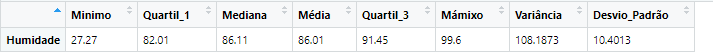
\includegraphics[scale=0.8]{tabela_humidade.png}
       \caption{Tabela com as medidas de localização e expressão da humidade.}
       \label{fig:logo}
    \end{figure}
    
\subsubsection{Gráfico para a variável comprimento de petala (Univariadas)}
\begin{figure}[h]
       \centering %centrar
        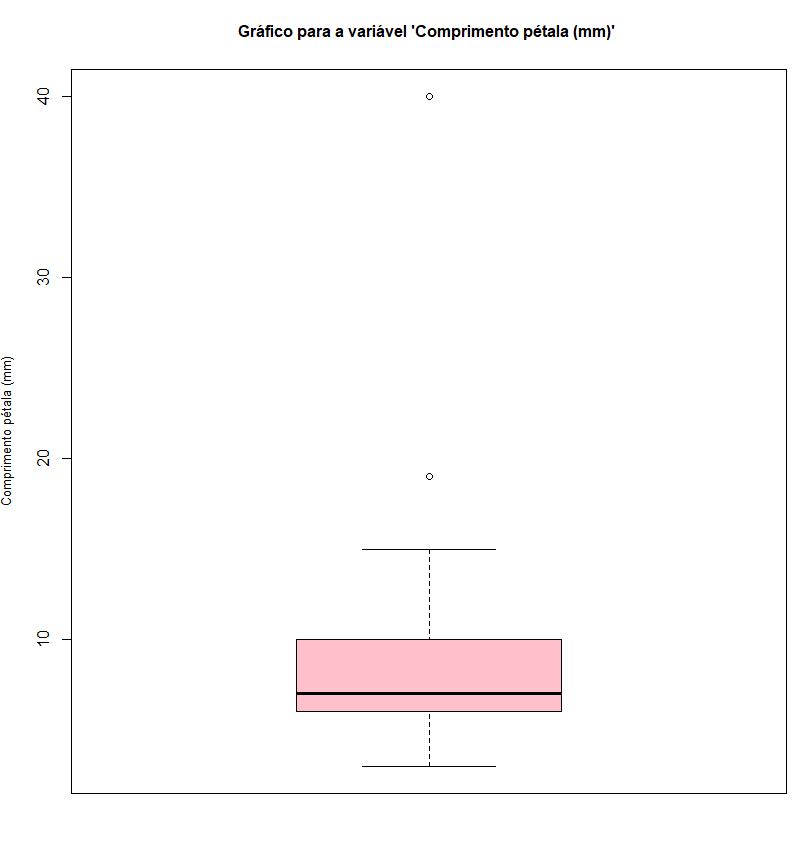
\includegraphics[scale=0.6]{gráfico comprimento pétala.png}
       \caption{Gráfico para a variável Comprimento.}
       \label{fig:logo}
    \end{figure}

\paragraph{}Neste gráfico podemos observar um valor minimo de 3.0 e máximo de 40.0, primeiro quartil de 6.0 e terceiro quartil de 10.0, mediana de 7.0, média de 8.13, variência de 14.5 e desvio padrão de 3.81

\begin{figure}[h]
       \centering %centrar
        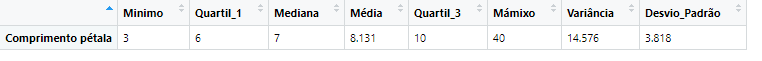
\includegraphics[scale=0.8]{tabela_compriento.png}
       \caption{Tabela com as medidas de localização e expressão do comprimento da pétala.}
       \label{fig:logo}
    \end{figure}
    
\paragraph{}

\paragraph{}



\subsubsection{Gráfico para a variável largura da petala (Univariadas)}
\begin{figure}[h]
       \centering %centrar
        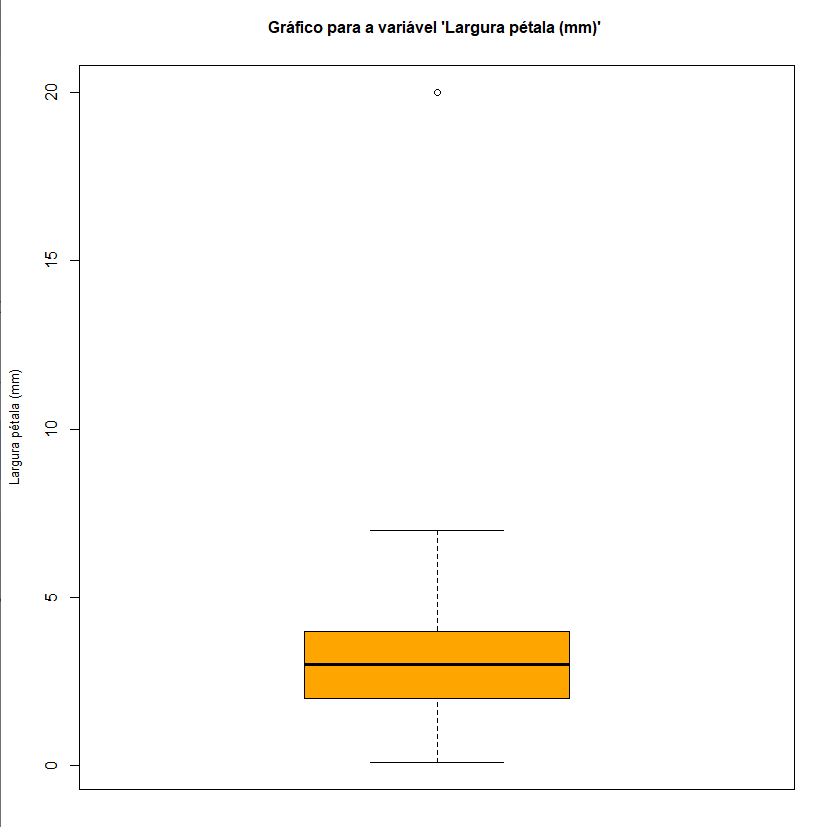
\includegraphics[scale=0.6]{gráfico largura pétala.png} 
       \caption{Gráfico para a variável largura.}
       \label{fig:logo}
    \end{figure}

\paragraph{}Neste gráfico podemos observar um valor minimo de 0.1 e máximo de 20.0, primeiro quartil de 2.0 e terceiro quartil de 4.0, mediana de 3.0, média de 2.96, variância de 4.09 e desvio padrão de 2.02


\begin{figure}[h]
       \centering %centrar
        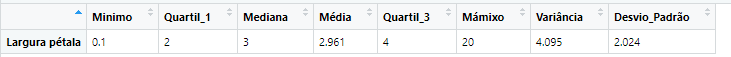
\includegraphics[scale=0.8]{tabela_largura.png}
       \caption{Tabela com as medidas de localização e expressão da largura da pétala.}
       \label{fig:logo}
    \end{figure}
    
\paragraph{}

\paragraph{}



\subsubsection{Gráfico para a variável do Nº de pétalas (Univariadas)}
\begin{figure}[h]
       \centering %centrar
        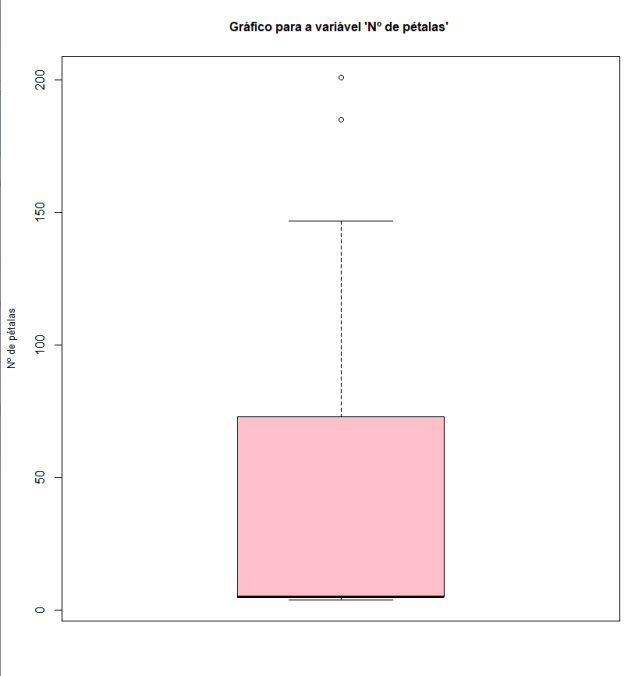
\includegraphics[scale=0.45]{grafico_no_de_petalas.png} 
       \caption{Gráfico circular para o Nº de pétalas.}
       \label{fig:logo}
    \end{figure}
    
\paragraph{}Neste gráfico podemos observar um valor minimo de 4.0 e máximo de 201.0, primeiro quartil de 5.0 e terceiro quartil de 72.25, mediana de 5.0, média de 2.96, variância de 2265.075 e desvio padrão de 47.59.

\begin{figure}[h]
       \centering %centrar
        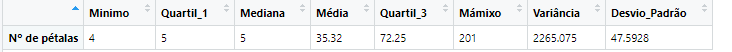
\includegraphics[scale=0.8]{tabela_nopetala.png} 
       \caption{Tabela com as medidas de localização e expressão do Nº de pétalas.}
       \label{fig:logo}
    \end{figure}
    
\paragraph{}
\paragraph{}

\subsubsection{Tabela de contingência entre comprimento e espécie.}
\begin{figure}[h]
       \centering %centrar
        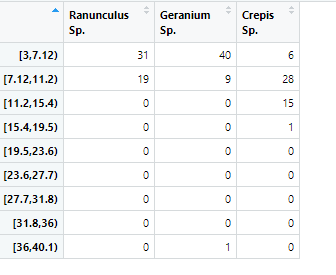
\includegraphics[scale=0.8]{tabela_do_comprimento_em_classe_com_especie.png} 
       \caption{Tabela de contingência entre comprimento e espécie.}
       \label{fig:logo}
    \end{figure}
    
\paragraph{}

\subsection{Associação de Cramer}

\begin{figure}[h]
       \centering %centrar
        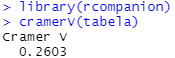
\includegraphics[scale=0.8]{associacao_de_cramer_entre_compriemento_e_especie.png} 
       \caption{Resultado da associação de cramer de acordo com  a tabela de contingencia.}
       \label{fig:logo}
    \end{figure}

Através do valor adquirido da análise da associação de Cramer, podemos afirmar que a associação entre a variável comprimento e a variável espécie é baixa.

\paragraph{}
\paragraph{}
\paragraph{}
\paragraph{}
\paragraph{}
\paragraph{}

\subsection{Correlação de Pearson}

\begin{figure}[h]
       \centering %centrar
        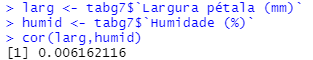
\includegraphics[scale=0.8]{correlacao_de_pearson_entre_largura_e_humidade.png} 
       \caption{Resultado da correlação de pearson entre largura e humidade.}
       \label{fig:logo}
    \end{figure}

Através do valor adquirido da análise da Correlação de Pearson, podemos afirmar que a relação entre a variável largura e a variável humidade é muito fraca e sem significância, ou seja, a largura das pétalas não interfere na percentagem de humidade.

\paragraph{}


\subsection{Estudo inferêncial}
\subsubsection{Primeira questão de investigação}
\textit{Pode-se considerar com uma confiança de 95$\%$ que a largura das pétalas  da cor amarela não é superior a 3 (mm).}
Pretende-se verificar se a média da largura da pétala da cor amarela é significativamente inferior a 3(mm), isto é \mu \leq 3 
\paragraph{} Como a variável em estudo está definida em uma escala quantitativa, o teste aplicado será o teste paramétrico de t-student, caso a largura da pétala provenha de uma população com distribuição normal.
\paragraph{} Como n=150, o teste de normalidade a aplicar é o teste de Kolmogorov-Smirnov com correção de Lilliefors.
\paragraph{} 
\textbf{Teste de Normalidade:}
\paragraph{}
\underline{Hipóteses:}
\paragraph{} H0: Largura das pétalas com a cor amarela provém de uma população com distribuição normal vs H1: Largura das pétalas com a cor amarela não provém de uma população com distribuição normal.

\paragraph{}
\paragraph{}
\paragraph{}
\paragraph{}

\paragraph{} \underline{Estatística de teste e significância:}

\begin{figure}[h]
       \centering %centrar
        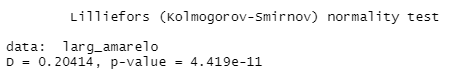
\includegraphics[scale=0.8]{teste_de_normalidade_para_a_1a_hipotese.png} 
       \caption{Teste de normalidade Kolmogorov-Smirnov com correção de Lilliefors}
       \label{fig:logo}
    \end{figure}
    
\paragraph{} D = 0.20414 
\paragraph{} p-value = \begin{math}4.419e^-^1^1\end{math}
\paragraph{} \underline{Decisão:}
\paragraph{} p-value = \begin{math}4.419e^-^1^1\end{math} \begin{math}<\end{math} 0.05 = \begin{math}\alpha\end{math} , logo rejeita-se a hipótese H0.
\paragraph{}\underline{Conclusão:}
\paragraph{}Para um nível de confiança de 95$\%$ a largura das pétalas com a cor amarela, não provém de uma população com distribuição normal(D = 0.20414 ; p-value = \begin{math}4.419e^-^1^1\end{math}).
\paragraph{}Como a variável não apresenta distribuição normal, não se pode usar o teste paramétrico ( t-student) sendo necessário recorrer à alternativa não paramétrica (teste de Wilcoxon).


\paragraph{}
\paragraph{}
\paragraph{}
\paragraph{}
\paragraph{}
\paragraph{}
\paragraph{}
\paragraph{}
\paragraph{}

\textbf{Teste de Wilcoxon:}
\paragraph{}
\underline{Hipóteses:}
\paragraph{} H0: Me \begin{math}\leq\end{math} 3 vs H1: Me \begin{math}>\end{math} 3


\paragraph{} \underline{Estatística de teste e significância:}

\begin{figure}[h]
       \centering %centrar
        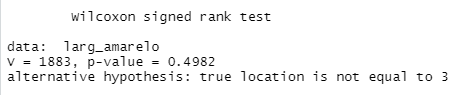
\includegraphics[scale=0.8]{teste_de_hipotese_1a_hipotese.png} 
       \caption{Teste não paramétrico de Wilcoxon}
       \label{fig:logo}
    \end{figure}
    
\paragraph{} V = 1883
\paragraph{} p-value = 0.4982
\paragraph{} \underline{Decisão:}
\paragraph{} p-value = 0.4982 \begin{math}>\end{math} 0.05 = \begin{math}\alpha\end{math}, logo não se rejeita a hipótese H0.
\paragraph{}\underline{Conclusão:}
\paragraph{}Para um nível de significância de 5$\%$ pode-se admitir que a largura das pétalas com a cor amarela não é superior a 3 (mm), logo a afirmação é verdadeira (V = 1883 ; p-value = 0.4982).
 
 
 \paragraph{}
 \paragraph{}
 \paragraph{}
 \paragraph{}
 \paragraph{}
 \paragraph{}
 \paragraph{}
 \paragraph{}
 
 \subsubsection{Segunda questão de investigação}
\textit{Pode-se considerar com uma confiança de 95$\%$ que a largura das pétalas  da cor roxa é pelo menos 4 (mm).}
Pretende-se verificar se a média da largura da pétala da cor roxa é significativamente maior ou igual a 4(mm), isto é \begin{math}\mu \geq \end{math} 4. 
\paragraph{} Como a variável em estudo está definida em uma escala quantitativa, o teste aplicado será o teste paramétrico de t-student, caso a largura da pétala provenha de uma população com distribuição normal.
\paragraph{} Como n=150, o teste de normalidade a aplicar é o teste de Kolmogorov-Smirnov com correção de Lilliefors.
\paragraph{} 
\textbf{Teste de Normalidade:}
\paragraph{}
\underline{Hipóteses:}
\paragraph{} H0: Largura das pétalas com a cor roxa provém de uma população com distribuição normal vs H1: Largura das pétalas com a cor roxa não provém de uma população com distribuição normal.

\paragraph{}

\paragraph{} \underline{Estatística de teste e significância:}

\begin{figure}[h]
       \centering %centrar
        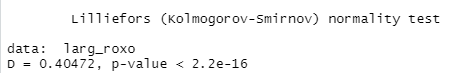
\includegraphics[scale=0.8]{teste_de_normalidade_para_a_2a_hipotese.png} 
       \caption{Teste de normalidade Kolmogorov-Smirnov com correção de Lilliefors}
       \label{fig:logo}
    \end{figure}
    
\paragraph{} D = 0.40472 
\paragraph{} p-value = \begin{math}2.2e^-^1^6\end{math}
\paragraph{} \underline{Decisão:}
\paragraph{} p-value = \begin{math}2.2e^-^1^6\end{math} \begin{math}<\end{math} 0.05 = \begin{math}\alpha\end{math} , logo rejeita-se a hipótese H0.
\paragraph{}\underline{Conclusão:}
\paragraph{}Para um nível de confiança de 95$\%$ a largura das pétalas com a cor roxa, não provém de uma população com distribuição normal(D = 0.40472 ; p-value = \begin{math}2.2e^-^1^6\end{math}).
\paragraph{}Como a variável não apresenta distribuição normal, não se pode usar o teste paramétrico ( t-student) sendo necessário recorrer à alternativa não paramétrica (teste de Wilcoxon).

\paragraph{}

\paragraph{}

\textbf{Teste de Wilcoxon:}
\paragraph{}
\underline{Hipóteses:}
\paragraph{} H0: Me \begin{math}\geq\end{math} 4 vs H1: Me \begin{math}<\end{math} 4


\paragraph{} \underline{Estatística de teste e significância:}

\begin{figure}[h]
       \centering %centrar
        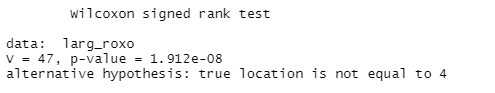
\includegraphics[scale=0.8]{teste_de_hipotese_2a_hipotese.png} 
       \caption{Teste não paramétrico de Wilcoxon}
       \label{fig:logo}
    \end{figure}
    
\paragraph{} V = 47
\paragraph{} p-value = \begin{math}1.912e^-^8\end{math}
\paragraph{} \underline{Decisão:}
\paragraph{} p-value = \begin{math}1.912e^-^8\end{math} \begin{math}<\end{math} 0.05 = \begin{math}\alpha\end{math}, logo rejeita-se a hipótese H0.
\paragraph{}
\paragraph{}
\paragraph{}\underline{Conclusão:}
\paragraph{}Para um nível de significância de 5$\%$ pode-se admitir que a largura das pétalas com a cor roxa não é superior a 4 (mm), logo a afirmação é falsa (V = 47 ; p-value = \begin{math}1.912e^-^8\end{math}).
 

 
\section{Conclusão}

Tendo em conta toda a informação e a vastidão deste trabalho, e tendo ainda a nossa perspetiva pessoal do mesmo, resta apenas acrescentar que este foi de extrema importância para a perceção dos conteúdos como também a assimilação dos mesmos. Assim sendo, após a realização do trabalho, todos os elementos constituintes do grupo conseguiram adquirir uma vasta aprendizagem sobre a linguagem do R-Studio e também sobre análises de gráficos e tabelas. Além do mais, também foi realizado a análise dos valores de duas variáveis quantitativas através da correlação de Pearson e a análise dos valores de uma variável qualitativa e uma variável quantitativa pela associação de Cramer. Entretanto houve a realização de duas questões de investigação na qual utilizámos o teste de normalidade Kolmogorov-Smirnov com correção de Lilliefors e o teste não paramétrico de Wilcoxon para ambas as investigações. Este projeto ajudou no quesito de ultrapassarmos as nossas dificuldades em relação a vários âmbitos da unidade curricular, tais como: R-Studio e testes de hipóteses. 


    %%% Bibliografia
    
    \begin{thebibliography}{}
    
    \bibitem{stackoverflow}
    (s.d.) Obtido de StackOverFlow stackoverflow.com
    \textit{R-Studio}
    
    \bibitem{overleaf}
   (s.d.) Obtido de overleaf www.overleaf.com \textit{Subscripts and superscripts}
   
    \bibitem{oeis}
   (s.d.) Obtido de oeis www.oeis.org \textit{List of LaTeX mathematical symbols}
    
    
    \end{thebibliography}


\end{document}
